%!TEX root = main.tex
\section{Simulation Study}
\label{sec:simulation}
We now evaluate the performance of the GFIC in a simulation experiment based on the dynamic panel example from the preceding section. 
The details of this simulation are similar those of \cite{AndrewsLu}.\footnote{Unlike \cite{AndrewsLu} we do not generate ``extra'' presample observations for use with estimators that include a lagged dependent variable. This is for two reasons. First, in real-world applications such additional observations would not be available. Second, we are explicitly interested in how the loss of time periods for estimation affects finite sample MSE.} 
The simulated covariates and error terms are jointly normal with mean zero and unit variance. 
Specifically,
	\begin{equation}
	\label{eq:covar}
		\left[\begin{array}{c}
			x_{i}\\
			\eta_i\\
			v_{i}
	 \end{array} \right]\sim \mbox{iid}\; N\left(\left[\begin{array}{c}0_T\\ 0\\ 0_T \end{array}\right] ,\left[\begin{array}{ccc}
	 	 I_T & \sigma_{x\eta}\iota_T&\sigma_{xv}\Gamma_T \\
	 		\sigma_{x\eta}\iota_T'& 1&0_T' \\
	 		\sigma_{xv}\Gamma_T'& 0_T&  I_T
	 \end{array}\right]\right)
	\end{equation}
where $0_m$ denotes an $m$-vector of zeros, $I_m$ the $(m\times m)$ identity matrix, $\iota_m$ an $m$-vector of ones, and $\Gamma_m$ an $m\times m$ matrix with ones on the subdiagonal and zeros elsewhere, namely
	\begin{equation}
		\Gamma_m = \left[\begin{array}{cc}
	 	0_{m-1}' & 0\\
	 	I_{m-1} & 0_{m-1}
	 \end{array}\right].
	\end{equation}
Under this covariance matrix structure, $\eta_i$ and $v_{i}$ are uncorrelated with each other, but both are correlated with $x_{i}$: $E[x_{it}\eta_i]=\sigma_{x\eta}$ and $x_{it}$ is predetermined but not strictly exogenous with respect to $v_{it}$. Specifically, $E[x_{it}v_{it-1}]=\sigma_{xv}$, while $E[x_{it}v_{is}]=0$ for $s\neq t-1$. 

We initialize the presample observations $y_{i0}$ to zero, the mean of their stationary distribution, and generate the remaining time periods according to 
$$y_{it} = \gamma y_{it-1} + \theta x_{it} + \eta_i + v_{it}$$
In the simulation we take $\theta = 0.5$, $\sigma_{x\eta}=0.2$ and vary $\gamma$, $\sigma_{xv}$, $T$ and $N$ over a grid.
Each grid point is based on 2000 simulation replications.

The first question is how the finite sample MSE of the 2SLS estimators of $\theta$ based on specifications LW, LS, W, and S (see Section \ref{sec:panel}) changes with $\gamma$ and $\sigma_{xv}$. 
Figures \ref{fig:best} and \ref{fig:advantage} present RMSE comparisons for these four estimators over a simulation grid with $\gamma, \sigma_{xv} \in \{0, 0.005, 0.01, \hdots, 0.195, 0.2\}$, $N \in \{250,500\}$, $T \in \{4,5\}$.\footnote{Taking $T$ no smaller than 4 ensures that MSE exists for all four estimators: the finite sample moments of the 2SLS estimator only exist up to the order of over-identification.} 
For each point in the parameter space, the color in Figure \ref{fig:best} indicates the estimator of $\theta$ with the \emph{lowest} finite sample RMSE. 
The saturation of the color indicates the relative difference in RMSE of the best estimator at that point measured against the second-best estimator: darker indicates a larger advantage; lighter indicates a smaller advantage. 
While Figure  \ref{fig:best} indicates \emph{which} estimator is best, Figure \ref{fig:advantage} indicates how much of an advantage in RMSE can be gained over the correct specification, LW. 
These plots indicate that, provided $\gamma$ and $\sigma_{xv}$ are not too large, there are potentially large gains to be had by intentionally using an incorrectly specified estimator. 
The question remains, can the GFIC identify such situations?

%%%%%%%%%%%%%%%%%%%%%%%%%%%%%%%%%%%%%%%%
\begin{figure}
\centering
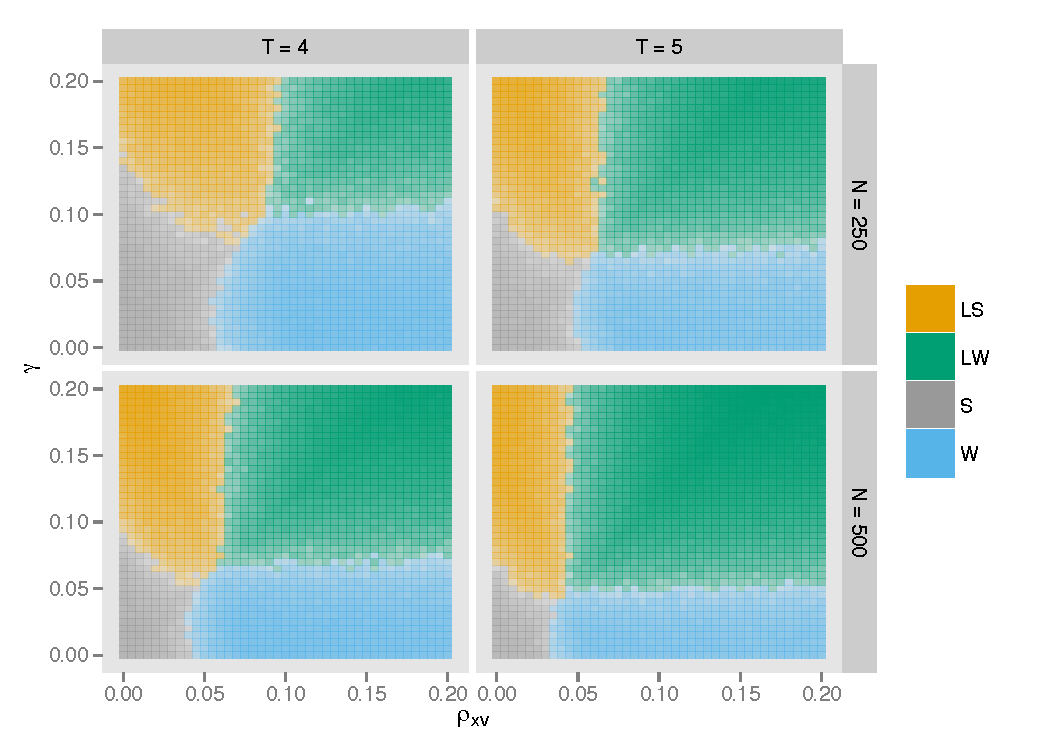
\includegraphics[scale = 0.8]{best_spec_vs_next_best}
\caption{ Minimum RMSE Specification at each combination of parameter values. Shading gives RMSE relative to second best specification.}
\label{fig:best}
\end{figure}

%%%%%%%%%%%%%%%%%%%%%%%%%%%%%%%%%%%%%%%%
\begin{figure}
\centering
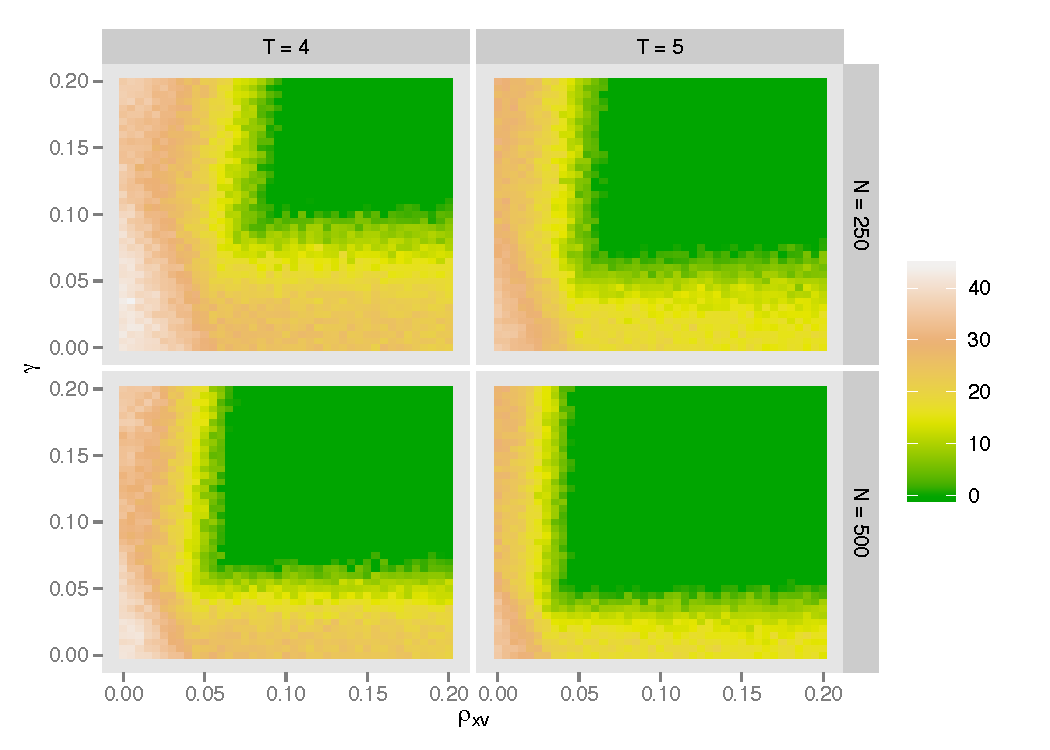
\includegraphics[scale = 0.8]{RMSE_advantage_vs_LW}
\caption{\% RMSE Advantage of Best Specification (vs.\ LW)}
\label{fig:advantage}
\end{figure}

%%%%%%%%%%%%%%%%%%%%%%%%%%%%%%%%%%%%%%%%

To provide a basis for comparison, we consider a number of other selection procedures. 
The first is a ``na\"{i}ve'' Downard J-test. 
To implement this procedure, we select the \emph{most restrictive} specification that is not rejected by the over-identifying restrictions test at a fixed significance level, either 5\% or 10\%. 
Specifically, we proceed as follows:
\begin{enumerate}
\item Use S unless the J-test rejects it. 
\item If S  is rejected, use W unless the J-test rejects it. 
\item If W is rejected, use LS unless the J-test rejects it. 
\item Only use LW if all others specifications are rejected.
\end{enumerate}
This procedure is ``na\"{i}ve'' because the significance thresholds are chosed arbitrarily rather than with a view towards some kind of selection optimality. 
We also consider the GMM model and moment selection criteria of \cite{AndrewsLu}: 
	\begin{eqnarray*}
	 \mbox{GMM-BIC} && J - (|c| - |b|) \log{n}\\
	 \mbox{GMM-AIC}&& J - 2(|c| - |b|)\\ 
	 \mbox{GMM-HQ} && J - 2.01 (|c| - |b|)  \log{\log{n}}
	\end{eqnarray*}
where $|b|$ is the number of parameters estimated, and $|c|$ the number of moment conditions used. 
Under certain assumptions, it can be shown that both the GMM-BIC and GMM-HQ are consistent: they select the maximal correctly specified estimator with probability approaching one in the limit. 
To implement these criteria, we calculate the J-test based on the optimal, two-step GMM estimator with a panel robust, heteroscedasticity-consistent, centered covariance matrix estimator for each specification.

To compare selection procedures we use the same simulation grid as above, namely $\gamma$ and $\sigma_{xv}$, namely $\gamma, \sigma_{xv} \in \{0, 0.005, 0.01, \hdots, 0.195, 0.20\}$.  
Again, each point on the simulation grid is calculated from 2000 simulation replications. 
Tables \ref{tab:rel} and \ref{tab:rmse} compare the performance of GFIC selection against each of the fixed specifications LW, LS, W, and S as well as the Downward J-test and the GMM moment and model selection criteria of \cite{AndrewsLu}. 
Table \ref{tab:rmse} gives average and maximum, i.e.\ worst-case, RMSE over the parameter space for $\gamma, \sigma_{xv}$ while Table \ref{tab:rel} gives \emph{relative} RMSE comparisons. Specifically, the values in the panel ``Average'' of Table \ref{tab:rel} tell how much larger, in percentage points, the average RMSE of a given estimator or selection procedure is than that of the pointwise oracle. 
The pointwise oracle is the infeasible procedure that uses the true minimum RMSE estimator at each point on the parameter grid. 
In contrast, the values in the panel ``Worst-Case'' of Table \ref{tab:rel} tell how much larger, in percentage points, the maximum RMSE of a given estimator or selection procedure is than that of the fixed specification LW. 
Over this parameter grid, LW is the minimax estimator.

Compared both to the fixed specifications and the other selection procedures, the GFIC performs well. 
In particular, it has a substantially lower average and worst-case RMSE than any of the other selection procedures.
Compared to simply using the correct specification, LW, the GFIC also performs relatively well. 
When $T$ and $N$ are small, the GFIC outperforms LW in average RMSE. 
As they grow it performs slightly worse, but only by a small amount.


\begin{table}[!tbp]
\begin{center}
\begin{tabular}{lrrrr}
\hline\hline
\multicolumn{1}{l}{Average}&\multicolumn{2}{c}{$N = 250$}&\multicolumn{2}{c}{$N = 500$}\\
&\multicolumn{1}{c}{$T=4$}&\multicolumn{1}{c}{$T=5$}&\multicolumn{1}{c}{$T=4$}&\multicolumn{1}{c}{$T=5$}\tabularnewline
\hline
LW&19&10&13& 7\tabularnewline
LS&30&44&54&79\tabularnewline
W&24&34&46&64\tabularnewline
S&31&50&64&94\tabularnewline
\hline
GFIC&17&13&15&10\tabularnewline
Downward J-test (10\%)&32&45&55&74\tabularnewline
Downward J-test (5\%)&31&47&57&79\tabularnewline
GMM-BIC&32&48&62&87\tabularnewline
GMM-HQ&32&46&57&77\tabularnewline
GMM-AIC&31&39&47&57\tabularnewline
\hline\\ \\ 

\hline\hline
\multicolumn{1}{l}{Worst-Case}&\multicolumn{2}{c}{$N = 250$}&\multicolumn{2}{c}{$N = 500$}\\
&\multicolumn{1}{c}{$T=4$}&\multicolumn{1}{c}{$T=5$}&\multicolumn{1}{c}{$T=4$}&\multicolumn{1}{c}{$T=5$}\tabularnewline
\hline
LW& 0& 0&  0&  0\tabularnewline
LS&42&81& 94&154\tabularnewline
W&49&88&105&158\tabularnewline
S&48&92&107&171\tabularnewline
\hline
GFIC& 3& 8&  6& 11\tabularnewline
Downward J-test (10\%)&43&78& 91&140\tabularnewline
Downward J-test (5\%)&45&83& 98&153\tabularnewline
GMM-BIC&48&89&106&168\tabularnewline
GMM-HQ&46&85&102&154\tabularnewline
GMM-AIC&39&68& 81&118\tabularnewline
\hline

\end{tabular}
\end{center}
\caption{Average and Worst-case RMSE Relative to Oracle (\% points)}
\label{tab:rel}
\end{table}

%%%%%%%%%%%%%%%%%%%%%%%%%%%%%%%%%%%%%%%%

\begin{table}[!tbp]
\begin{center}
\begin{tabular}{lrrrr}
\hline\hline
\multicolumn{1}{l}{Average}&\multicolumn{2}{c}{$N = 250$}&\multicolumn{2}{c}{$N = 500$}\\
&\multicolumn{1}{c}{$T=4$}&\multicolumn{1}{c}{$T=5$}&\multicolumn{1}{c}{$T=4$}&\multicolumn{1}{c}{$T=5$}\tabularnewline
\hline
LW&0.073&0.057&0.051&0.040\tabularnewline
LS&0.079&0.074&0.070&0.066\tabularnewline
W&0.075&0.069&0.066&0.061\tabularnewline
S&0.080&0.077&0.074&0.072\tabularnewline
\hline
GFIC&0.071&0.058&0.052&0.041\tabularnewline
Downward J-test (10\%)&0.080&0.074&0.070&0.065\tabularnewline
Downward J-test (5\%)&0.080&0.075&0.071&0.067\tabularnewline
GMM-BIC&0.080&0.076&0.073&0.069\tabularnewline
GMM-HQ&0.080&0.075&0.071&0.066\tabularnewline
GMM-AIC&0.080&0.071&0.066&0.058\tabularnewline
\hline\\ \\

\hline\hline
\multicolumn{1}{l}{Worst-Case}&\multicolumn{2}{c}{$N = 250$}&\multicolumn{2}{c}{$N = 500$}\\
&\multicolumn{1}{c}{$T=4$}&\multicolumn{1}{c}{$T=5$}&\multicolumn{1}{c}{$T=4$}&\multicolumn{1}{c}{$T=5$}\tabularnewline
\hline
LW&0.084&0.064&0.059&0.045\tabularnewline
LS&0.120&0.116&0.115&0.113\tabularnewline
W&0.125&0.120&0.122&0.115\tabularnewline
S&0.125&0.123&0.122&0.121\tabularnewline
\hline
GFIC&0.087&0.069&0.063&0.049\tabularnewline
Downward J-test (10\%)&0.120&0.114&0.113&0.107\tabularnewline
Downward J-test (5\%)&0.122&0.117&0.117&0.113\tabularnewline
GMM-BIC&0.125&0.121&0.122&0.119\tabularnewline
GMM-HQ&0.123&0.118&0.120&0.113\tabularnewline
GMM-AIC&0.117&0.107&0.107&0.097\tabularnewline
\hline
\end{tabular}
\end{center}
\caption{Average and Worst-case RMSE.}
\label{tab:rmse}
\end{table}
%%%%%%%%%%%%%%%%%%%%%%%%%%%%%%%%%%%%%%%%


